\chapter{Fundamentos Teóricos}
Este capítulo tiene como objetivo introducir y explicar los fundamentos teóricos en los que se basan los métodos empleados en el trabajo, así como de su relevancia para la resolución del problema planteado.

\section{Aprendizaje Automático}
El Aprendizaje Automático, o \textit{Machine Learning} (ML) \cite{abu-mostafa_learning_2012, mitchell_introduction_1997, 6284961}, es una rama de la Inteligencia Artificial (IA) que se enfoca en el desarrollo de programas informáticos para resolver tareas complejas donde no existe una solución analítica directa. Es decir, no es posible describir un algoritmo que, dados los datos de entrada, los transforme en los datos de salida esperados. En estos casos, a menudo se carece de un conocimiento detallado y completo del problema, lo que puede intentarse compensar mediante el uso de datos relacionados. Estos datos pueden emplearse para obtener una solución empírica, donde el sistema \say{aprende} de ellos. A partir de los datos, se extraen patrones o reglas que permiten construir un algoritmo aproximado, conocido como modelo, capaz de resolver la tarea incluso cuando se enfrenta a datos no vistos previamente. Formalmente, se puede definir que un programa aprende de la experiencia $E$ en relación con una clase de tareas $T$ y una métrica de rendimiento $P$ si su rendimiento en las tareas $T$, medido por $P$, mejora con la experiencia $E$. Este aprendizaje se clasifica en dos grandes grupos: supervisado y no supervisado. En el aprendizaje supervisado, se dispone tanto de los datos de entrada como de las salidas correctas correspondientes, mientras que en el aprendizaje no supervisado solo se tienen los datos de entrada y se espera que el programa identifique patrones dentro de estos.

En términos generales, es factible aplicar ML en problemas que cumplen con alguna de las siguientes condiciones: (a) cuando se dispone de extensas bases de datos que permiten extraer patrones intrínsecos, lo que se conoce como minería de datos o \textit{data mining} \cite{alma991006986149704990}; (b) en aquellos problemas cuyos dominios no están bien definidos o en los que resulta difícil para un humano describirlos de manera precisa para desarrollar un algoritmo, como ocurre en tareas de detección de objetos en imágenes; y (c) en dominios en los que el sistema debe adaptarse de forma dinámica a condiciones cambiantes \cite{mitchell_introduction_1997}.

En el aprendizaje supervisado se distinguen dos tareas fundamentales: la clasificación y la regresión, cuya principal diferencia radica en la naturaleza de la variable de salida. En las tareas de clasificación, cada ejemplo de entrada se asigna a una categoría discreta. Esto implica que el modelo debe aprender a identificar y etiquetar cada muestra dentro de un conjunto finito de clases. Por otro lado, en las tareas de regresión el objetivo es predecir un valor numérico continuo. En este caso, la salida del modelo puede tomar cualquier valor dentro de un rango determinado.

A partir de las descripciones previas, se puede concluir que es viable aplicar técnicas de ML al problema en cuestión. En este caso, se dispone de datos de entrada, que corresponden a los huesos de la sínfisis del pubis, y de datos de salida, representados por los atributos de cada hueso clasificados según las nueve categorías del método de Todd. Además, aunque los antropólogos forenses poseen el conocimiento experto necesario para identificar estos patrones, dicho conocimiento no puede expresarse de manera analítica. Por ello, el problema se enmarca dentro del aprendizaje supervisado, siendo específicamente un problema de clasificación, ya que es necesario asignar a cada hueso los atributos correspondientes a las categorías establecidas por el método de Todd.

\section{Aprendizaje Profundo}
\label{section:DL}
El aprendizaje profundo (\textit{Deep Learning}, DL) \cite{Goodfellow-et-al-2016, lecun_deep_2015, schmidhuber_deep_2015} es una subdisciplina de ML en la que el modelo se encarga de aprender y extraer de manera automática las características relevantes a partir de los datos del problema. Esta aproximación contrasta con otras técnicas de ML en las que las características son diseñadas manualmente o \textit{handcrafted} por expertos que utilizan su conocimiento específico del dominio. Se ha demostrado que, para problemas de alta complejidad, las características extraídas de forma automática tienden a ser más efectivas y eficientes en comparación con aquellas obtenidas manualmente.

El modelo predominante en el ámbito del DL es la red neuronal artificial (\textit{Artificial Neural Network}, ANN) \cite{bishop_ANN, ripley_ANN}, compuesta por nodos de procesamiento, denominados \say{neuronas}{\interfootnotelinepenalty=10000 \footnote{Aunque su denominación es bioinspirada en la corteza visual del cerebro, estos modelos no simulan de forma precisa el funcionamiento biológico neuronal.}}, interconectados en diferentes capas. La red se estructura con una capa de entrada, que recibe los datos en bruto, seguida de una o varias capas ocultas encargadas de aprender y extraer progresivamente las características relevantes, y una capa de salida. En las capas iniciales se capturan atributos de bajo nivel, mientras que las subsiguientes permiten obtener representaciones más abstractas y de alto nivel, facilitando la solución del problema planteado. La cantidad de capas en una ANN define su profundidad, lo que justifica el término aprendizaje profundo: en general, a mayor número de capas, se logra un aprendizaje más detallado y eficaz. Un ejemplo clásico de una ANN se ilustra en la Figura \ref{fig:annExample}, donde se diferencia claramente entre una red superficial y una red profunda.

\begin{figure}[h]
    \centering
    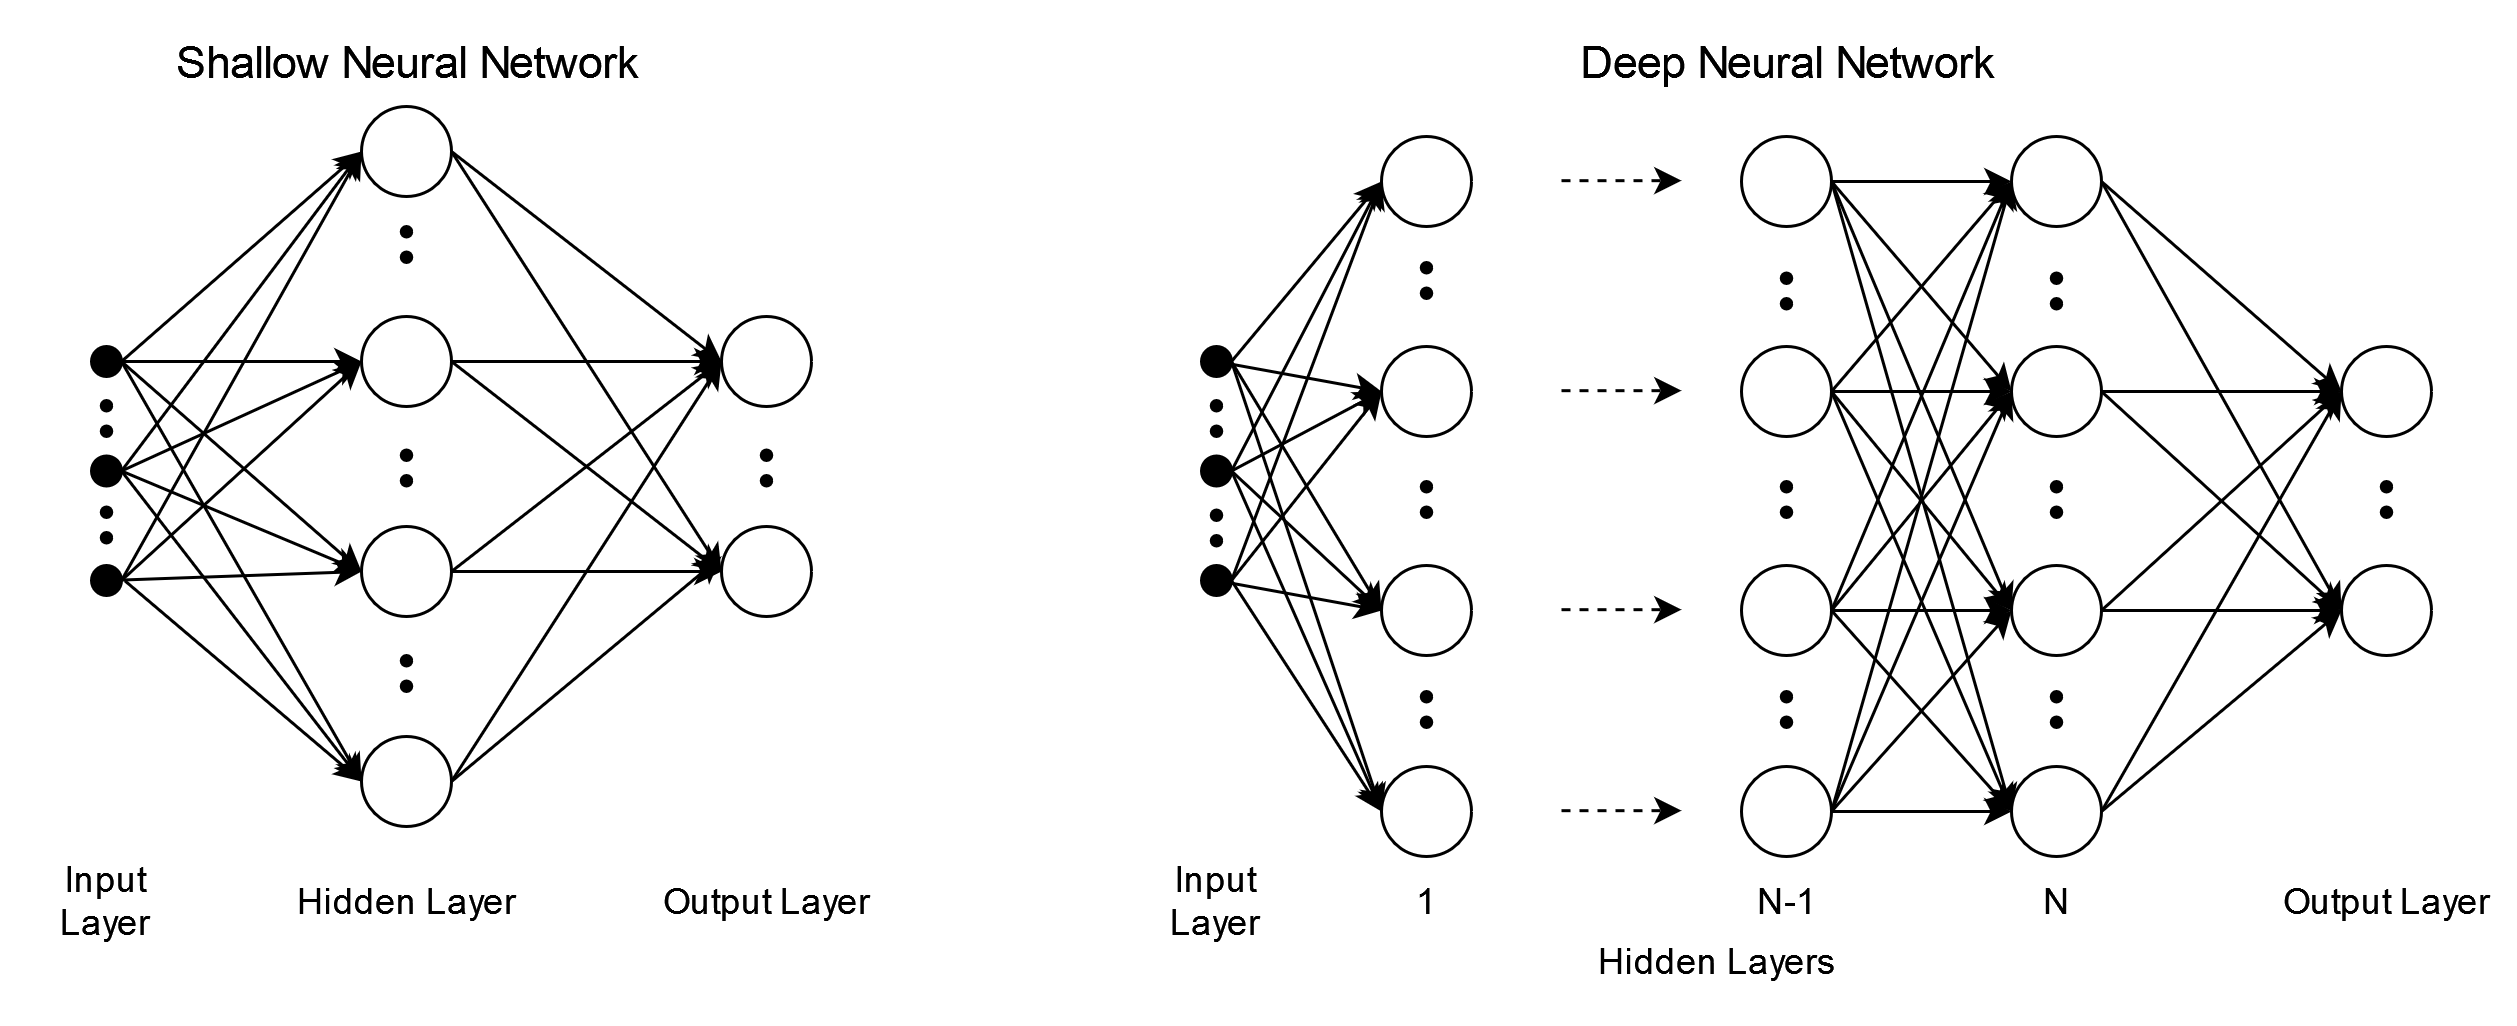
\includegraphics[width=\linewidth]{figures/2_theory/neuralNetDiagram.png}
    \caption[Ejemplos de la estructura de una ANN]{Ejemplos típicos de la estructura de una ANN, en este caso se tiene una red superficial o \textit{shallow} y una profunda o \textit{deep} \cite{annPictureSource}.}
    \label{fig:annExample}
\end{figure}

Cada neurona, como se ha descrito, recibe múltiples valores de entrada y produce un valor de salida que sirve como entrada para la siguiente capa. Además, cada neurona incorpora una función de activación no lineal\footnote{Si la función fuera lineal, toda la red se reduciría a una simple neurona, resultando en un modelo lineal, ya que la combinación de funciones lineales produce otra función lineal.}, la cual transforma las entradas en el valor de salida que se transmite. Esta función actúa de manera similar a un umbral, permitiendo que la red amplifique ciertas señales y suprima otras, en función de lo que se desea aprender. Dicho comportamiento se logra mediante la asignación de pesos a cada entrada de la neurona, junto con un valor adicional conocido como sesgo o bias. La modificación de los pesos y el sesgo permite ajustar la magnitud de la señal procesada por la función de activación. Un ejemplo visual de una neurona artificial se puede observar en la Figura \ref{fig:artificialNeuronExample}.

Existen numerosas funciones de activación, aunque las más comunes y ampliamente utilizadas incluyen la función sigmoidal o logística, la tangente hiperbólica y la ReLU (\textit{Rectified Linear Unit}). La elección de una función específica dependerá de la naturaleza y los requerimientos del problema a resolver.

\begin{figure}[h]
    \centering
    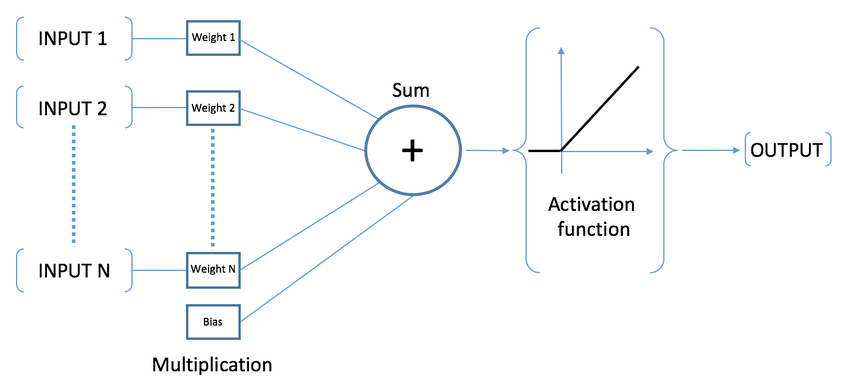
\includegraphics[width=\linewidth]{figures/2_theory/artificialNeuron.png}
    \caption[Ejemplo de una neurona artificial]{Ejemplo de una neurona artificial, los datos de entrada son multiplicados por los pesos y su resultado, junto con el sesgo (o \textit{bias}), son combinados linealmente. A continuación, son transformados por la función no lineal para proporcionar el valor salida de la neurona \cite{artificialNeuron}.}
    \label{fig:artificialNeuronExample}
\end{figure}

El aprendizaje en una ANN consiste esencialmente en ajustar los pesos y el sesgo de cada neurona para que, tras ser procesados por la función de activación, se puedan extraer y transformar las características más relevantes de los datos. El proceso inicia con la propagación hacia adelante (\textit{forward propagation}), en la cual los datos atraviesan la red desde la capa de entrada, pasando por las capas ocultas, hasta llegar a la capa de salida. Durante esta fase, se calculan los valores de salida de cada neurona, lo que finalmente permite obtener un resultado global de la red.

En este punto entra en juego la función de pérdida o error, cuya finalidad es medir qué tan bien ha aprendido la red. Existen diversas funciones de pérdida, y la elección de una en particular depende del tipo de problema y del enfoque de aprendizaje utilizado. A partir del valor de error obtenido, se aplica el algoritmo de retropropagación (\textit{backpropagation}), el cual calcula las derivadas de los pesos y sesgos respecto a dicho error. Posteriormente, mediante el uso de un algoritmo de optimización (\textit{optimizer}), se recalculan los valores de los pesos con el objetivo de minimizar el error de manera iterativa.

Este procedimiento, conocido como entrenamiento, permite que la red ajuste sus parámetros de manera progresiva hasta alcanzar un modelo que represente de manera óptima los patrones de los datos. Sin embargo, este enfoque de aprendizaje presenta un desafío fundamental en ML: el sobreentrenamiento u \textit{overfitting}. Este fenómeno ocurre cuando el modelo se ajusta excesivamente a los datos de entrenamiento, perdiendo capacidad de generalización. En tales casos, la red logra un error muy bajo en el conjunto de entrenamiento, pero su desempeño se deteriora considerablemente cuando se enfrenta a datos nuevos o no vistos previamente.

\subsection{Redes Neuronales Convolucionales}
\label{cnnDescription}
Las redes neuronales convolucionales (\textit{Convolutional Neural Network}, CNN) \cite{lecun_backpropagation_1989, leCUM_CNN} son un tipo de red neuronal artificial ampliamente utilizada en tareas de procesamiento, clasificación y segmentación de imágenes. Además, su aplicación se ha extendido a otras áreas como el procesamiento de texto, sonidos y, más recientemente, el análisis de superficies tridimensionales. A diferencia de una ANN tradicional, en la que todas las neuronas están completamente conectadas entre sí, una CNN introduce dos tipos adicionales de capas: capas convolucionales y capas de \textit{pooling}.

La estructura básica de una CNN puede visualizarse en la Figura \ref{fig:cnnExample}, donde se observa que la red está dividida en dos partes fundamentales. La primera parte está compuesta exclusivamente por capas convolucionales y de \textit{pooling}, cuyo propósito es extraer características relevantes de los datos de entrada. En la segunda parte, la estructura se asemeja a una ANN clásica, en la que las características extraídas se combinan de manera no lineal, permitiendo que la red realice tareas como la clasificación o detección de patrones dentro de los datos procesados.

\begin{figure}[h]
    \centering
    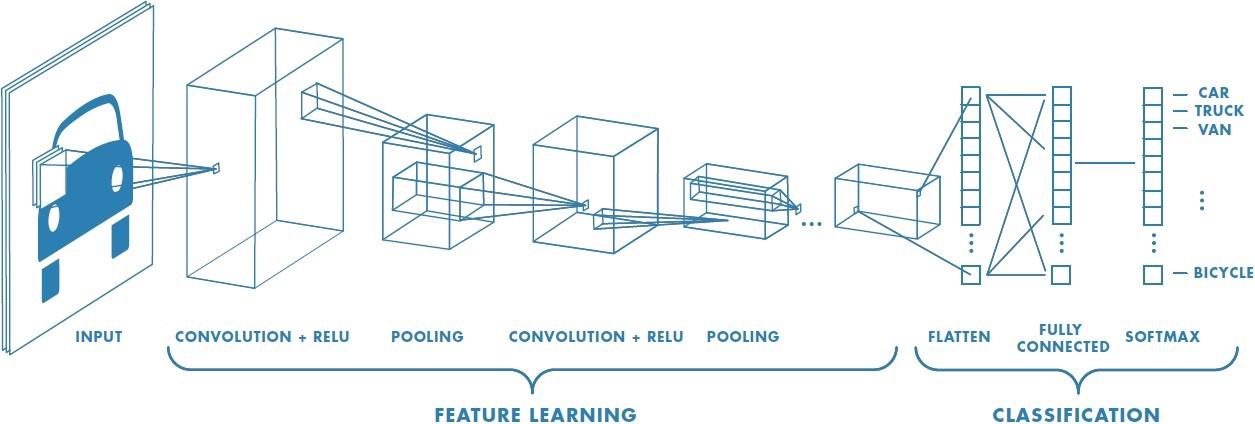
\includegraphics[width=\linewidth]{figures/2_theory/cnnExample.jpeg}
    \caption[Estructura básica de una red neuronal convolucional]{Estructura básica de una CNN donde se pueden apreciar las diferentes capas que la componen \cite{prabhu_understanding_2019}.}
    \label{fig:cnnExample}
\end{figure}

\subsection{Capa convolucional}
La capa convolucional es el elemento central de una CNN. A diferencia de una ANN clásica, en la que cada neurona está conectada con todas las neuronas de las capas vecinas, en una capa convolucional cada neurona está conectada únicamente a un vecindario local de neuronas. Esto es posible gracias a la operación de convolución, la cual permite procesar la imagen de entrada de manera eficiente\footnote{De aquí en adelante, se explicará el funcionamiento de la CNN clásica aplicada a imágenes, aunque su principio es similar en otros tipos de datos.}.

Una convolución consiste en un producto punto entre dos matrices (ver Figura \ref{fig:convolution} para una representación visual):
\begin{itemize}
    \item El \textit{kernel} (filtro o núcleo de la convolución), que es un conjunto de pesos que la red puede aprender y modificar.
    \item El campo receptivo (\textit{receptive field}), que es un fragmento de la imagen con el que el \textit{kernel} se multiplica en un momento dado.
\end{itemize}

El \textit{kernel} se desplaza por la imagen, comenzando en una esquina y moviéndose a través de filas y columnas de píxeles hasta recorrer toda la imagen. La matriz resultante de esta operación se procesa mediante una función no lineal, al igual que en una neurona clásica, y genera un mapa de características o mapa de activación, que servirá como entrada para la siguiente capa de la red.

Gracias a este proceso, la CNN puede capturar patrones espaciales y temporales en los datos mediante la aplicación de filtros relevantes. En las primeras capas convolucionales, la red aprende características de bajo nivel (como bordes y texturas), que luego se combinan en las capas siguientes para identificar características de alto nivel (como formas y estructuras más complejas).

Sin embargo, la aplicación directa de la convolución sobre una imagen reduce el tamaño del mapa de activación debido a la propia naturaleza del operador. Para mitigar esto, se pueden emplear técnicas como:
\begin{itemize}
    \item Relleno (\textit{padding}): Se añaden píxeles alrededor de la imagen utilizando información ya presente en ella, lo que permite mantener la misma dimensionalidad en la salida.
    \item Saltos (\textit{strides}): Se modifica el número de píxeles que avanza el kernel en cada paso, lo que puede reducir aún más la salida de la capa convolucional.
\end{itemize}

\begin{figure}[h]
    \centering
    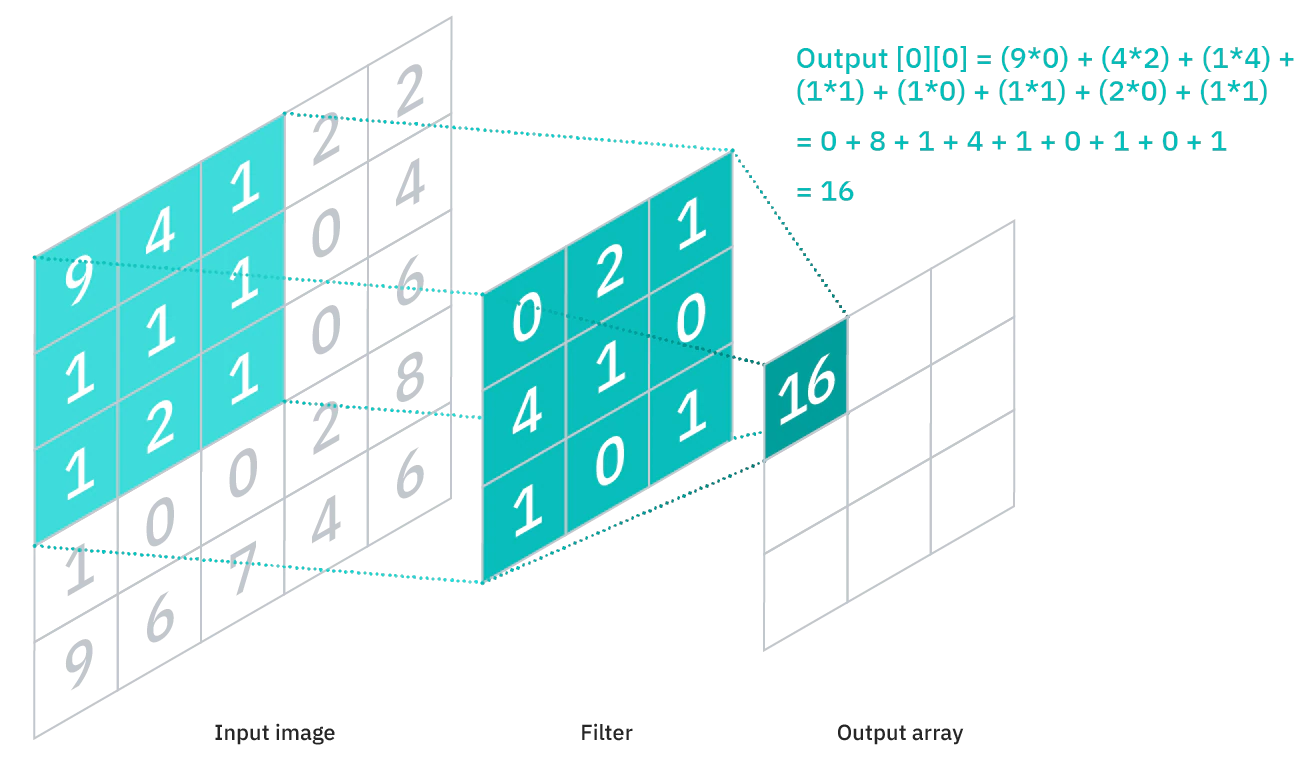
\includegraphics[width=\linewidth]{figures/2_theory/convolution.png}
    \caption[Ejemplo del operador de convolución]{Ejemplo de una convolución 2D con un \textit{kernel} $3 \times 3$. El campo receptivo para la neurona actual es la submatriz $3\times3$ de la imagen original con la que se está multiplicando el \textit{kernel} \cite{noauthor_what_2021}.}
    \label{fig:convolution}
\end{figure}

\subsection{Capa de \textit{pooling}}

Las capas de \textit{pooling} tienen como único objetivo reducir la dimensionalidad del mapa de activación generado por las capas convolucionales. Por ello, se insertan inmediatamente después de estas. Aunque las propias convoluciones pueden disminuir la resolución de los mapas de activación, el \textit{pooling} ofrece una forma más controlada de lograrlo y, además, mejora la extracción de características.

El \textit{pooling}, al igual que la convolución, utiliza un filtro o ventana que se desplaza a lo largo de los datos con un determinado salto (\textit{stride}). Sin embargo, en lugar de aplicar una operación de convolución, se realizan operaciones de reducción, como:
\begin{itemize}
    \item \textit{Max Pooling}: Se selecciona el valor máximo dentro de la ventana, lo que ayuda a preservar las características más relevantes y genera mayor invarianza a la traslación.
    \item \textit{Average Pooling}: Se calcula el promedio de los valores dentro de la ventana, lo que suaviza la salida y reduce el ruido en los datos.
\end{itemize}
La Figura \ref{fig:poolingExample} ilustra cómo funcionan estas operaciones.

\begin{figure}[h]
    \centering
    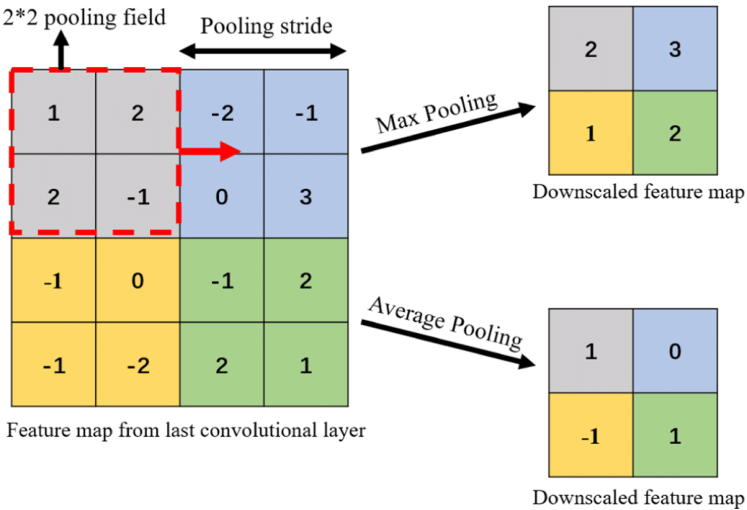
\includegraphics[width=\linewidth]{figures/2_theory/poolingExample.png}
    \caption[Ejemplo del operador de pooling]{Ejemplo de las operaciones de \textit{pooling} con un filtro $2\times2$ y \textit{stride} 2 \cite{pooling}.}
    \label{fig:poolingExample}
\end{figure}

Las capas convolucionales y de \textit{pooling} en conjunto conforman la sección de extracción de características en una CNN. Dependiendo de la complejidad del problema, el número de estas capas puede variarse para asegurar que la red extraiga las características esenciales necesarias para el aprendizaje.

\subsection{Capa totalmente conectada}
Las capas totalmente conectadas (\textit{fully connected} o \textit{dense layers}) aparecen después de las capas de convolución y \textit{pooling}, y constituyen la parte final de una CNN. Estas capas siguen la estructura de una ANN clásica, donde cada neurona está conectada con todas las neuronas de las capas adyacentes. Tomando como entrada las características extraídas y de ellas aprenden combinaciones no lineales. Gracias a esto, la red neuronal puede cumplir su objetivo, ya sea la clasificación o la regresión.

La última capa densa es la salida de toda la red. En esta etapa, se evalúa la función de pérdida, que mide la diferencia entre la predicción del modelo y la realidad. Luego, mediante \textit{backpropagation} y un algoritmo de optimización, los pesos de todas las neuronas de la red se ajustan durante el entrenamiento para minimizar el error.

\subsection{Regularización}
\label{subsection:regularization}
Como se ha comentado anteriormente, tanto las ANNs como las CNNs son propensas al fenómeno de sobreentrenamiento u \textit{overfitting}. La regularización es un método utilizado para combatir este fenómeno y en esencia lo que se quiere es controlar la complejidad del modelo, ya sea alterando los datos, el número de parámetros o el funcionamiento de la red. En general, la regularización es cualquier modificación que se puede realizar al modelo para que generalice mejor.

Se compone de múltiples técnicas diferentes, pero las más relevantes y utilizadas en CNNs son: La normalización, \textit{data augmentation}, la inicialización de los pesos y \textit{dropout}.

\subsubsection{Normalización}

\begin{figure}[h]
    \centering
    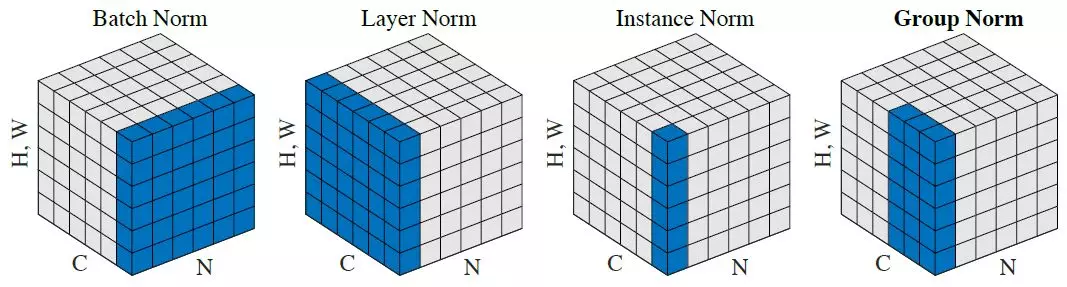
\includegraphics[width=\linewidth]{figures/2_theory/normTypes.png}
    \caption[Tipos de normalización]{Diferentes tipos de normalización. \textbf{H,W} indican la altura y anchura de la imagen, \textbf{C} indica los canales y \textbf{N} el número de lotes \cite{wu2018group}.}
    \label{fig:normTypes}
\end{figure}

La normalización es una técnica que estandariza los datos de manera que el valor medio de los mismos sea cercano a 0, con una desviación estándar cercana a 1, empíricamente se ha demostrado que esto mejora el rendimiento de las redes, pues evita que los pesos posean valores muy grandes, lo que afecta el cálculo de gradientes. 

Por lo general la normalización se aplica a las capas convolucionales de la red y la manera típica de utilizarla es haciendo uso de la normalización por lotes o \textit{batch normalization}, en donde se aplica la estandarización a una característica $i$-ésima de entrada calculando la media y desviación típica de todas las características $i$-ésimas del lote. Existe también la normalización por capa o \textit{layer normalization} que aplica la media y desviación típica por cada capa independiente del lote, la normalización por grupo o \textit{group normalization} que aplica la normalización a un grupo de canales pero no toda la capa entera. Por último se tiene la normalización por instancia o \textit{instance normalization} que normaliza cada canal por separado. El uso de un tipo u otro de normalización depende de la tarea a cumplir, pues se sabe que empíricamente diferentes tipos producen mejores modelos en diferentes problemas. Un ejemplo visual de todos los tipos de normalización se puede observar en la Figura \ref{fig:normTypes}. 

\subsubsection{\textit{Data Augmentation}}
El aumento de datos o \textit{data augmentation}, es una técnica para aumentar la cantidad de datos que se poseen de manera artificial, significa que, se generan nuevos datos de los ya presentes mediante la aplicación de transformaciones aleatorias pero realistas. Por ejemplo, escalados no uniformes de la imagen, rotaciones, traslaciones, adición de ruido o transformaciones de perspectiva. De esta manera se poseen más muestras de entrenamiento diferentes, lo que reduce la posibilidad de \textit{overfitting} porque la red tendrá más datos con los que trabajar y las modificaciones realizadas ayudan a la red a tener una idea más general de lo que se está aprendiendo.

\subsubsection{Inicialización de los pesos}
Como ha sido mencionado, las ANNs y CNNs utilizan pesos y sesgos en cada neurona, que son modificados en el entrenamiento por un algoritmo de optimización. Estos algoritmos necesitan un valor inicial que sea diferente de 0 al comienzo de dicho entrenamiento para funcionar, y la elección de estos valores afecta de gran forma al entrenamiento de la red, por lo tanto, se considera también como una técnica de regularización.

Se pueden inicializar los valores de forma aleatoria utilizando una distribución normal o uniforme que no toma en cuenta ningún parámetro de la red. Aún así, existen diversas heurísticas que se han desarrollado sobre los años que se ha comprobado mejoran el entrenamiento de los modelos. Por ejemplo, se tiene la inicialización Xavier \cite{glorot2010understanding} que parte de una distribución uniforme pero que toma en cuenta la cantidad de entradas que posee cada neurona, por lo que la inicialización está parcialmente guiada por la densidad de las capas. Otra inicialización heurística se denomina Kaiming \cite{he2015delving} y genera los valores por medio de una distribución normal acotada por el número de entradas de la capa.

\subsubsection{\textit{Dropout}}
La técnica de abandono o \textit{dropout} consiste en apagar o desactivar temporalmente cierta cantidad de neuronas en las capas totalmente conectadas de forma aleatoria durante el proceso de entrenamiento. La aplicación del \textit{dropout} hace que la red generalice mejor, pues las neuronas en una capa totalmente conectada tienden a generar una codependencia entre ellas, es decir, que ciertas neuronas se adaptan para contrarrestar los errores de otras neuronas y debido a que estos errores dependen de los datos de entrenamiento, no se generalizará bien para nuevos datos. Por lo tanto el \textit{dropout} permite evitar estas codependencias e impulsar el poder individual de cada neurona, lo cual aumenta el poder de generalización de la red.

\section{Clasificación Multietiqueta}
Como se ha descrito anteriormente, la clasificación emplea una variable de salida asociada a una variable discreta. Sin embargo, existe una extensión de esta idea en la que, para cada variable de entrada, pueden existir múltiples categorías asociadas que no se solapan entre sí. Este enfoque se conoce como clasificación multietiqueta (o multi-label classification).

En un problema de clasificación tradicional, cada instancia pertenece exclusivamente a una única clase dentro de un conjunto de categorías predefinidas. Por ejemplo, en la clasificación de imágenes de animales, un modelo puede etiquetar una imagen como \say{perro} o \say{gato}, pero no ambas a la vez. En contraste, en la clasificación multietiqueta, cada instancia puede estar asociada con múltiples categorías simultáneamente.

Un ejemplo común de este tipo de clasificación se encuentra en el etiquetado de imágenes en redes sociales, donde una misma foto puede contener etiquetas como \say{persona}, \say{playa} y \say{atardecer}. De manera similar, en el procesamiento de textos, un documento puede clasificarse dentro de varias categorías temáticas, como \say{tecnología}, \say{negocios} y \say{ciencia}, si su contenido abarca múltiples áreas.

Entre los algoritmos de ML más utilizados para la clasificación multietiqueta destacan los árboles de decisión, los métodos de vecinos más próximos, las máquinas de vectores de soporte (SVM) y las redes neuronales. En particular, las redes neuronales han logrado mejoras en el aprendizaje cuando se utiliza este método \cite{ranjan_hyperface_2019}.

Dado que el problema en cuestión involucra la clasificación de huesos de la sínfisis del pubis según las nueve categorías del método de Todd, es posible abordarlo mediante un enfoque de clasificación multietiqueta, donde bien se utilicen todas o algunas de las características en un único modelo de DL en vez de un modelo por cada característica.

\section{Grad-CAM}
El mapeo de activación de clase ponderado por gradiente (\textit{Gradient-weighted Class Activation Mapping}, Grad-CAM) \cite{selvaraju_grad_cam_2017} es una técnica ampliamente utilizada para interpretar el funcionamiento de las CNNs en tareas de clasificación de imágenes. Su propósito es identificar qué regiones de una imagen influyen en la decisión del modelo, proporcionando así una representación visual del proceso de clasificación.

Grad-CAM genera mapas de calor que destacan la relevancia de cada píxel en relación con una clase específica, generalmente aplicándose en la última capa convolucional de la red. Para ello, combina de manera lineal las activaciones de dicha capa, ponderadas por el gradiente de la salida correspondiente. Este cálculo permite resaltar las áreas de la imagen que impactan positiva o negativamente en la predicción del modelo. Finalmente, se conservan únicamente las contribuciones positivas, es decir, aquellas que refuerzan la decisión del modelo en favor de la clase seleccionada.

Por ejemplo observar la Figura \ref{fig__grad_cam} donde se tiene una fotografía de un perro y un gato (\ref{fig__grad_cam__og}). Si se estudia la clase \say{gato} con Grad-CAM, se obtiene un mapa de calor que indica que partes de la imagen han contribuido a que el modelo detecte al gato (\ref{fig__grad_cam__cat}). De igual forma si se estudia la clase \say{perro}, se obtiene un mapa de calor distinto indicando que partes influenciaron la detección del perro (\ref{fig__grad_cam__dog}).

La principal ventaja de Grad-CAM radica en su capacidad para generar explicaciones visuales, lo que facilita la comprensión de los factores que influyeron en la decisión de la red respecto a una clase específica. Además, este método es altamente versátil, ya que puede aplicarse a una amplia variedad de redes neuronales convolucionales sin necesidad de modificar su estructura, y su cálculo es relativamente sencillo.

Sin embargo, una de sus principales limitaciones es la dificultad para evaluar la precisión de las explicaciones generadas. En algunos casos, la interpretación de los mapas de calor puede no ser intuitiva o carecer de sentido lógico, lo que impide obtener resultados claramente interpretables \cite{molnar2025}.

\begin{figure}[!h]  
    \centering
    \begin{subfigure}{0.28\textwidth}
        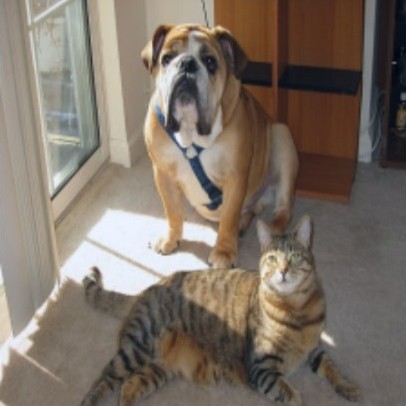
\includegraphics[width=\textwidth]{figures/2_theory/grad_cam__og.jpg}
        \begin{minipage}{.1cm}
            \vfill
            \end{minipage}
        \caption{Fotografía original.}
        \label{fig__grad_cam__og}
    \end{subfigure}
    \begin{subfigure}{0.28\textwidth}
        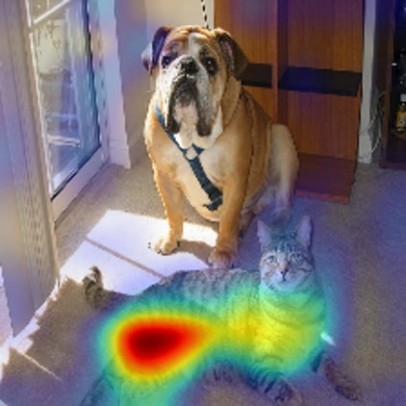
\includegraphics[width=\textwidth]{figures/2_theory/grad_cam__cat.jpg}
        \caption{Mapa de activación para la clase \say{gato}.}
        \label{fig__grad_cam__cat}
    \end{subfigure}  
    \begin{subfigure}{0.28\textwidth}
        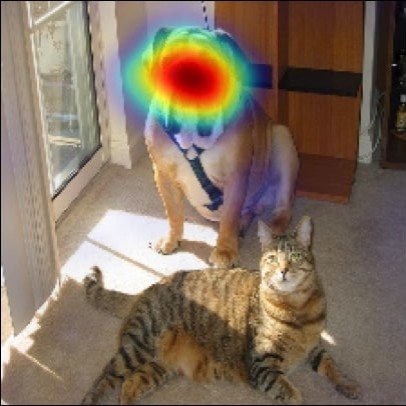
\includegraphics[width=\textwidth]{figures/2_theory/grad_cam__dog.jpg}
        \caption{Mapa de activación para la clase \say{perro}.}
        \label{fig__grad_cam__dog}
    \end{subfigure}    
    \caption{Ejemplo de funcionamiento de Grad-CAM \cite{selvaraju_grad_cam_2017}.}
    \label{fig__grad_cam}          
\end{figure}

\section{Búsqueda de Arquitectura Neuronal}
La búsqueda de arquitectura neuronal (\textit{Neural Architecture Search}, NAS) \cite{zoph_neural_2017} es un método que automatiza la generación de la estructura de una red neuronal. A diferencia de obtener una estructura por medio de conocimiento experto, se utilizan algoritmos para explorar e identificar la mejor arquitectura de red neuronal para una tarea específica. Este enfoque automatizado ayuda a optimizar el rendimiento, la velocidad y la eficacia \cite{ultralytics_busqueda_nas}.

El enfoque consiste en definir un espacio de búsqueda de posibles arquitecturas de red, establecer una estrategia para explorar este espacio y evaluar el rendimiento de cada arquitectura. Este proceso iterativo permite a NAS descubrir arquitecturas muy eficaces para tareas específicas que podrían no ser diseñadas intuitivamente por los humanos, y que a menudo igualan o superan las mismas tanto en exactitud como en uso de recursos y tamaño \cite{poyser_neural_2024}.

Si bien existen actualmente una gran cantidad de algoritmos NAS, estos se pueden clasificar en distintos grupos dependiendo de la estrategia utilizada para la exploración del espacio de búsqueda \cite{baymurzina_review_2022, white_neural_2023}.

\subsection{Métodos de búsqueda}
\subsubsection{Por métodos evolutivos}
Los métodos evolutivos o de \textit{neuroevolution} hacen uso de algoritmos evolutivos para la generación de la estructura de la red. La idea principal es la de ir modificando iterativamente la arquitectura por medio de una población de redes candidatas por el uso de operadores de cruce y mutación para incrementar su valor de evaluación o \textit{fitness}, en cada siguiente iteración se van cruzando las redes con el mejor \textit{fitness} para obtener descendientes hasta que se obtenga un valor deseado de \textit{fitness} o se llegue a un criterio de para definido. Notablemente, la función de optimización no tiene por qué ser diferenciable, por lo que resultan particularmente útiles para optimización multi objetivo. 

Este método ha demostrado obtener redes con la misma efectividad que las obtenidas por humanos, pero esto viene con el conocido alto coste computacional que requieren los algoritmos evolutivos. Adicionalmente existen los costos computacionales de entrenar desde cero cada integrante de la población por cada iteración para determinar su \textit{fitness}.

\subsubsection{Por optimización bayesiana}
La optimización bayesiana es un método para encontrar la mejor arquitectura de red utilizando un modelo probabilístico sustituto. Este modelo predice el rendimiento de distintas arquitecturas y se actualiza iterativamente a medida que se recopilan nuevos datos. Para decidir qué arquitecturas probar, se usa una función de adquisición, que equilibra la exploración (probar opciones nuevas) y la explotación (refinar las mejores opciones encontradas). Una vez seleccionada una arquitectura prometedora, se evalúa su rendimiento real y se incorpora esta información en el modelo. Este proceso se repite hasta alcanzar un criterio de parada definido.

Este método es muy popular en NAS debido a que, en comparación con otros métodos, obtiene arquitecturas buenas en pocas iteraciones y es capaz de soportar espacios de búsqueda complejos, aunque está limitada en escalabilidad y en la paralelización de la búsqueda.

\subsubsection{Por aprendizaje por refuerzo}
El método de aprendizaje por refuerzo (\textit{Reinforcement Learning}, RL) intenta mejorar la búsqueda en el espacio de soluciones utilizando un modelo controlador conocido como un \say{agente} que realiza una \say{acción} muestreando una arquitectura y recibe una \say{recompensa} que es alguna métrica de validación de la red neuronal, como por ejemplo el \textit{accuracy} de la misma. En este paradigma, el agente iterativamente aprende a generar la arquitectura que genere las mejores recompensas basándose en algoritmos de RL basados en políticas o en valores.

Este método se ha demostrado capaz de obtener redes con las mismas capacidades que las diseñadas a mano, con el mayor cuello de botella siendo la necesidad de reentrenar cada modelo para la siguiente iteración, aunque se han desarrollado variantes que permiten modificar una red parcialmente entrenada para ahorrar tiempo de cómputo.

\subsubsection{Por pesos compartidos}
Esta familia de métodos surge por los costos computacionales producidos por la necesidad de reentrenar cada red candidata desde cero. La solución propuesta permite que pesos de las neuronas estén compartidos entre diferentes redes.

Se puede realizar por el uso de una SuperRed (\textit{SuperNet}), donde un agente LSTM selecciona una subred para ser entrenada como una solución candidata al problema. De  esta forma las neuronas que son comunes para las distintas subredes van actualizándose en cada entrenamiento al mismo tiempo que el agente LSTM va aprendiendo qué subredes son las mejores para el problema. Si bien reduce substancialmente el tiempo de cómputo, poseen alto uso de memoria y necesitan ser cuidadosamente tuneadas, de lo contrario los pesos pueden interferirse entre sí provocando un colapso en su desempeño.

Otro método, denominado Búsqueda de Arquitectura Diferenciable (\textit{Differentiable Architecture Search}, DART), en vez de tratar el espacio de búsqueda como algo discreto, se relaja para volverlo continuo representando las operaciones candidatas (por ejemplo: convoluciones, pooling y saltos en las conexiones) como sumas ponderadas, permitiendo así hacer uso del \textit{backpropagation} para optimizar tanto los pesos de la red neuronal como la arquitectura misma. Reducen el tiempo de cómputo en comparación con otros métodos, pero de igual forma poseen un alto uso de memoria y son susceptibles a converger en operaciones demasiado simples.

\subsubsection{Por búsqueda aleatoria}
Este método es el más básico e ingenuo de los utilizados, se trata de seleccionar arquitecturas al azar de las posibilidades del espacio de búsqueda y quedarse con la que obtenga la mejor puntuación en la métrica seleccionada. Aunque se trate de un concepto bastante sencillo y que por lo general estos métodos se utilizan como bases para comparar los métodos anteriormente mencionados, se pueden obtener muy buenas arquitecturas si se ha diseñado el espacio de búsqueda correctamente.

\subsection{Espacios de búsqueda}
Hay que tomar en cuenta que las estrategias de búsqueda son independientes del espacio de búsqueda, la elección este espacio puede afectar drásticamente el desempeño de la red resultante, representa un importante compromiso entre el sesgo humano y la eficiencia de la búsqueda: si el tamaño del espacio de búsqueda es pequeño e incluye muchas decisiones seleccionadas manualmente, los algoritmos NAS tendrán más facilidad para encontrar una arquitectura de alto rendimiento. Por otro lado, si el espacio de búsqueda es grande y contiene bloques de construcción más primitivos, un algoritmo NAS necesitará ejecutarse durante más tiempo, pero existe la posibilidad de descubrir arquitecturas novedosas \cite{white_neural_2023}.

\subsubsection{Espacios de búsqueda basados en cadenas}
Los espacios de búsqueda basados en cadenas, como el nombre sugiere, tienen una topología sencilla: encadenar capas de operaciones para generar la arquitectura de la red. Son conceptualmente simples, lo cual los hacen fáciles de diseñar e implementar. También permiten que se encuentren con facilidad arquitecturas eficaces, pero por tener una topología tan sencilla es menos probable que se obtengan diseños de arquitecturas verdaderamente novedosas.

\subsubsection{Espacios de búsqueda basados en celdas}
Los espacios de búsqueda basados en celdas toma inspiración en el hecho que la mayoría de las arquitecturas del estado del arte para CNNs consisten en patrones repetidos múltiples veces, como por ejemplo, los bloques residuales en la familia de redes ResNets. Por lo tanto, en vez de intentar generar toda la red desde cero, se enfoca en buscar \say{celdas} relativamente pequeñas y apilarlas en secuencia para formar la arquitectura de la red. Cabe destacar que la forma de la red a gran escala se encuentra predefinida, pero cada bloque se puede componer de diferentes \say{celdas}. Son muy populares y pueden obtenerse con rapidez, pero como la macroestructura se encuentra ya fija, no permiten mucha expresividad y variación de las arquitecturas que se obtienen.

\subsubsection{Espacios de búsqueda jerárquicos}
A diferencia de los otros tipos de espacios de búsqueda, en lo que todo el diseño de la arquitectura es \say{plano} o diseñado en una sola capa, los espacios de búsqueda jerárquicos poseen múltiples niveles en los que se va definiendo la estructura de la red desde los parámetros más generales hasta los más específicos. Son extremadamente expresivos, permiten obtener redes complejas y diversas, además de que al tener la jerarquía se hace más efectivo la búsqueda del espacio lo que lo hace más eficiente también. Por otro lado, son bastante más complicados de diseñar e implementar.

\section{Representaciones 3D en \textit{Deep Learning}}
\label{3d_reps}
Las CNNs fueron originalmente diseñadas para procesar imágenes, es decir, datos bidimensionales organizados en estructuras regulares. Como consecuencia, aún no existe un consenso sobre la mejor manera de representar modelos tridimensionales en el contexto del \textit{Deep Learning}, dado que este tipo de datos suele presentar estructuras irregulares, lo que dificulta la adaptación de los métodos tradicionales. Además, la investigación en esta área es relativamente reciente.

No obstante, el desarrollo de dispositivos más accesibles para la digitalización y generación de modelos 3D a partir de objetos físicos, junto con el crecimiento en la cantidad de modelos tridimensionales generados por ordenador y la instauración del concurso anual \textit{3D Shape Retrieval Challenge} (SHREC) \cite{noauthor_shrec_nodate, noauthor_3dor2024_nodate}, han impulsado la exploración de diversas estrategias para representar información tridimensional de manera que pueda ser procesada mediante DL. Cada una de estas estrategias presenta ventajas y limitaciones particulares.

En la literatura, se han identificado cinco principales categorías de representaciones tridimensionales: datos en bruto, sólidos, superficies, estructuras de alto nivel y datos de múltiples vistas (véase Figura \ref{fig:3dTaxonomy}). Esta clasificación fue propuesta inicialmente por Ahmed et al. \cite{ahmed_survey_2019} y posteriormente ampliada por Gezawa et al. \cite{gezawa_review_2020} y Muzahid et al. \cite{muzahid_deep_2024}.

\begin{figure}[h]
    \centering
    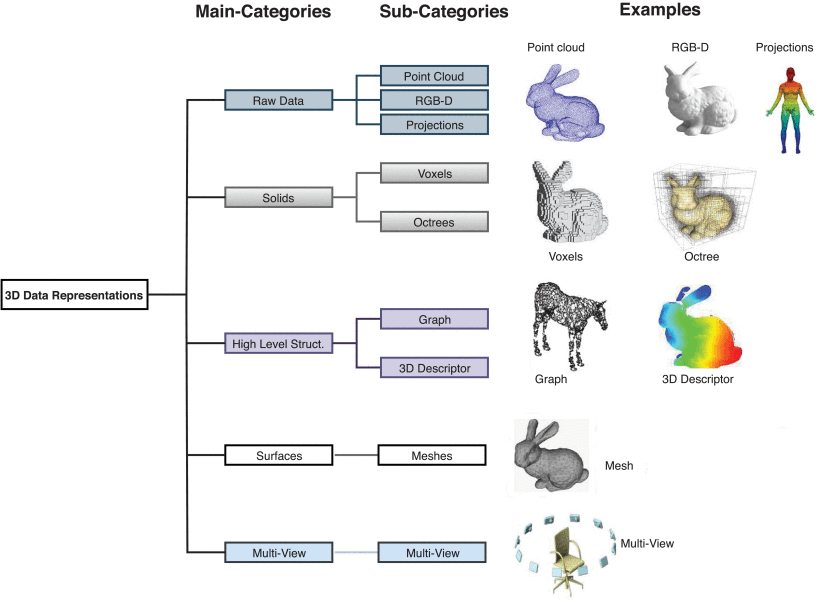
\includegraphics[width=\linewidth]{figures/2_theory/3Dtaxonomy.png}
    \caption[Taxonomía de las representaciones 3D para Deep Learning]{Taxonomía de las diferentes técnicas actuales en DL utilizadas para representar datos tridimensionales \cite{gezawa_review_2020}.}
    \label{fig:3dTaxonomy}
\end{figure}

\subsection{Datos en bruto}
Los datos en bruto corresponden a la información tridimensional obtenida directamente mediante métodos de escaneo, sin aplicar transformaciones significativas. Estos datos pueden ser capturados mediante dispositivos como el Microsoft Kinect o escáneres de luz estructurada, lo que permite representar la geometría de los objetos con un alto grado de fidelidad.

\subsubsection{Nube de Puntos}
La nube de puntos es una representación tridimensional compuesta por un conjunto de puntos sin estructura explícita, definidos por coordenadas espaciales, ya sea en un sistema cartesiano u otro sistema de referencia. Esta técnica tiene su origen en la fotogrametría y, más recientemente, en el escaneo mediante tecnología LiDAR.

Su principal ventaja radica en su facilidad de obtención y su fidelidad con los datos originales, ya que es una de las representaciones más cercanas a la captura en bruto. Sin embargo, su procesamiento es complejo debido a la ausencia de información sobre la conectividad entre los puntos, lo que puede generar ambigüedades en la forma real del objeto. Además, las nubes de puntos suelen contener datos incompletos o ruidosos, lo que dificulta la distinción entre información relevante y elementos espurios.

\subsubsection{Datos RGB-D}
Los datos RGB-D constituyen una representación tridimensional en la que se combina información cromática en formato RGB con un canal adicional de profundidad (D), que indica la distancia de cada píxel al sensor. Esta técnica fue popularizada por el Microsoft Kinect y proporciona una representación en 2.5D del objeto.

La principal ventaja de los datos RGB-D es la facilidad con la que pueden ser adquiridos y procesados, lo que ha permitido la creación de numerosos \textit{datasets} para su análisis. No obstante, su principal limitación radica en la falta de información geométrica completa, ya que no capturan la estructura tridimensional completa del objeto, restringiendo su aplicabilidad en tareas que requieren un modelado detallado de la forma.

\subsubsection{Proyecciones}
Las proyecciones permiten mapear información tridimensional en un plano bidimensional mediante la generación de vistas proyectadas del objeto. Estas proyecciones pueden ser de distintos tipos, siendo las cilíndricas y esféricas las más utilizadas debido a su invarianza frente a rotaciones alrededor del eje principal.

Entre sus ventajas destaca su capacidad para conservar las características más relevantes de la superficie 3D proyectada, además de facilitar el uso de modelos preentrenados en imágenes bidimensionales. Sin embargo, su aplicación en tareas complejas relacionadas con superficies tridimensionales es limitada, ya que la transformación a 2D conlleva la pérdida de información topológica fundamental.

\subsection{Sólidos}
Las representaciones de sólidos en modelos tridimensionales proporcionan detalles sobre el espacio que ocupa un objeto en tres dimensiones, es decir, indican si una región específica del espacio está ocupada o vacía por el objeto en cuestión. Estas representaciones se enfocan principalmente en describir tanto la estructura interna como la ocupación espacial del objeto.

\subsubsection{Vóxeles}
La representación mediante vóxeles puede pensarse como una cuadrícula regular en tres dimensiones, en la cual el modelo 3D está distribuido. Además, la información del punto de vista puede codificarse clasificando los vóxeles como visibles o no visibles desde dicho punto de vista.

Aunque los vóxeles ofrecen una representación completa del modelo, la necesidad de representar tanto las áreas ocupadas como las vacías del volumen conlleva un uso excesivo de memoria, lo que hace inviable su utilización en modelos de alta resolución debido a la gran demanda de recursos.

\subsubsection{Árbol octal}
El árbol octal es una representación más eficiente en comparación con la de vóxeles, ya que, en lugar de utilizar una cuadrícula regular, el tamaño de los vóxeles es variable. Los árboles octales modelan la información tridimensional mediante una estructura de datos jerárquica en forma de árbol, que describe la ocupación del objeto dentro de la escena 3D. Esta representación se basa en la descomposición recursiva de la escena en cubos, cada uno de los cuales tiene 8 subceldas (hijos) que pueden estar dentro o fuera del objeto.

Su principal ventaja radica en su mayor eficiencia en comparación con los vóxeles, permitiendo representar los detalles con mayor precisión y generar modelos de alta resolución. Sin embargo, su principal desventaja es la incapacidad para mantener con exactitud la geometría de ciertos objetos 3D, como es el caso de la suavidad en las superficies.

\subsection{Estructuras de alto nivel}
En tareas como la clasificación y la recuperación de formas tridimensionales, es necesario contar con representaciones que sean tanto concisas como detalladas de los modelos 3D. Estas representaciones permiten describir un objeto de manera que sea representativo de una categoría específica.

\subsubsection{Descriptor 3D}
Los descriptores 3D son representaciones simplificadas, generalmente creadas manualmente o \textit{handcrafted}, de los modelos 3D, que capturan las características geométricas o topológicas del objeto. Estos descriptores pueden derivarse de varias propiedades, como la geometría, la topología, la superficie, la textura o una combinación de todas ellas. Se pueden considerar como una \say{firma} que caracteriza de manera única un modelo 3D.

La principal ventaja es que facilitan el procesamiento y la computación de modelos 3D, siendo especialmente útiles en tareas de comparación, análisis y recuperación de formas tridimensionales, particularmente en contextos de aprendizaje no supervisado. Sin embargo, su mayor desventaja es que su utilidad disminuye en tareas de aprendizaje supervisado. Esto se debe a que el descriptor extrae características de los datos en bruto, lo que implica una abstracción adicional sobre los datos del modelo 3D. En un modelo supervisado, se estaría aprendiendo a partir de una abstracción de una abstracción, lo que puede resultar en la pérdida de información si la representación es demasiado simple o abstracta.

\subsubsection{Grafos}
La representación mediante grafos permite resumir la información tridimensional conectando las diversas formas a través de nodos y aristas. En este enfoque, los nodos del grafo corresponden a los vértices del modelo, mientras que las aristas representan las conexiones entre estos vértices. Los grafos pueden ser dirigidos o no dirigidos.

Dentro del contexto de redes neuronales sobre grafos, existen dos tipos principales de métodos: filtrado espectral y filtrado espacial. Los métodos de filtrado espectral se basan en la descomposición en valores y vectores propios de la laplaciana del grafo, utilizando este análisis para definir un operador similar a la convolución. En contraste, los métodos de filtrado espacial emplean filtros de paso alto y bajo como combinaciones lineales de las capas de la red. El proceso de aprendizaje se centra en el vecindario local de cada vértice, aplicando funciones no lineales a cada nodo del grafo.

Esta representación tiene la ventaja de que se puede aplicar a mallas 3D, y han mostrado resultados prometedores en diversas aplicaciones. Sin embargo, su principal desventaja radica en los altos costos computacionales y la dependencia del grafo base utilizado, lo que limita la capacidad de generalización entre diferentes dominios, haciendo que la transferencia de conocimientos entre ellos no siempre sea consistente.

\subsection{Superficies}
Este tipo de representación describe la superficie que cubre las partes internas de un objeto 3D mediante un conjunto de polígonos. Las superficies presentan la ventaja de ser simples, fáciles de procesar y de dibujar, ya que todas las superficies pueden representarse mediante ecuaciones lineales. Existen varios métodos de representación superficial, tales como las subdivisiones, las mallas paramétricas e implícitas. Sin embargo, la representación más popular y utilizada en el ámbito de DL es la malla poligonal, especialmente la malla triangular.

\subsubsection{Malla 3D}
Las mallas 3D están formadas por una combinación de vértices, aristas y caras. Cada vértice tiene asociada una lista de conectividad que indica cómo se conectan entre sí, y esta lista puede interpretarse como el conjunto de aristas que, a su vez, describen las caras de la malla.

La principal ventaja de las mallas 3D es su amplia adopción y relevancia en los gráficos por ordenador, tanto para almacenar descripciones de modelos 3D como para su visualización. No obstante, debido a su irregularidad y complejidad, el estudio de su aplicación en tareas de aprendizaje profundo no se había abordado satisfactoriamente hasta tiempos recientes. Hoy en día, se trata de una de las áreas más novedosas, con modelos que han alcanzado resultados satisfactorios, aunque con un alto consumo de recursos computacionales.

\subsection{Múltiples vistas}
Esta representación consiste en modelar un objeto 3D mediante un conjunto de imágenes tomadas desde diferentes puntos de vista, utilizando técnicas tradicionales de gráficos por ordenador. Posteriormente, estas imágenes se emplean como entradas para una CNN convencional.

La principal ventaja de esta representación es que permite aprovechar todas las técnicas y métodos ya existentes para CNNs basadas en imágenes, lo que facilita la utilización de modelos de alta resolución. Sin embargo, su mayor desventaja radica en la dificultad de determinar el número adecuado de puntos de vista a utilizar, así como en la pérdida de información que ocurre cuando partes del modelo 3D se solapan entre sí y quedan ocultas desde ciertos ángulos. Además, esta representación no conserva las propiedades geométricas intrínsecas del modelo 3D, y el uso de múltiples vistas conlleva un alto costo computacional.